\documentclass[11pt]{article}
\usepackage[utf8]{inputenc}
\usepackage{amsmath}
\usepackage{amsfonts,epsfig}
\usepackage[hyphens]{url}
\usepackage[colorlinks,citecolor=blue,urlcolor=blue]{hyperref}
\usepackage{microtype}
\usepackage{breakurl}
\usepackage{comment}

% \usepackage[
% scale=.875,
% stdmathitalics=true,
% stdmathdigits=true]{lucimatx}
\linespread{1.02}

\usepackage{relsize}
\usepackage{fancyvrb}
\usepackage{amssymb}
%%% Document layout, margins
\usepackage{geometry}
\geometry{letterpaper, textwidth=6.5in, textheight=9in, marginparsep=1em}
%%% Section headings
\usepackage{sectsty}
\usepackage{caption}
\usepackage{subcaption}
% \usepackage[export]{adjustbox}
\usepackage[normalem]{ulem}
\sectionfont{\sffamily\bfseries\upshape\large}
\subsectionfont{\sffamily\bfseries\upshape\normalsize}
\subsubsectionfont{\sffamily\mdseries\upshape\normalsize}
\makeatletter
\renewcommand\@seccntformat[1]{\csname the#1\endcsname.\quad}
\makeatother\renewcommand{\bibitem}{\vskip 2pt\par\hangindent\parindent\hskip-\parindent}

\makeatletter
\def\@maketitle{%
  \begin{center}%
  \let \footnote \thanks
    {\large \@title \par}%
    {\normalsize
      \begin{tabular}[t]{c}%
        \@author
      \end{tabular}\par}%
    {\small \@date}%
  \end{center}%
}
\makeatother


\title{\bf Monitoring mixing of iterative simulation using split R-hat and effective sample size\footnote{We thank the National Science Foundation, Office of Naval Research, Institute for Education Sciences, Sloan Foundation, and Academy of Finland (grant 313122) for partial support of this work. Much of the material in this paper is copied from Gelman et al.\ (2013).}\vspace{.1in}}
\author{Andrew Gelman\footnote{Department of Statistics and Department of Political Science, Columbia University.} \and Bob Carpenter\footnote{Institute for Social and Economic Research and Policy, Columbia University.} \and Aki Vehtari\footnote{Helsinki Institute for Information Technology HIIT,
           Department of Computer Science, Aalto University,
           Finland}}
\date{19 April 2018\vspace{-.1in}}
\begin{document}\sloppy
\maketitle
\thispagestyle{empty}

\begin{abstract}
We review split-$\widehat{R}$ and effective sample size, two tools we use to routinely monitor the convergence of iterative simulations.  These methods have already been published in the Stan manual and the third edition of {\em Bayesian Data Analysis} but it is convenient to have them here in a short article. This article includes some additional details and corrections. 
\end{abstract}

\section{The problem}\label{intro}

Iterative simulation, particularly Markov chain Monte Carlo (MCMC), is increasingly popular in statistics (Brooks et al., 2011), especially in Bayesian applications where the goal is to represent posterior inference using a sample of posterior draws.  Iterative simulation algorithms in common use typically can be proven to converge to the target distribution as the number of draws approaches infinity, but convergence is only approximate for any finite number of draws.

Following usual Bayesian practice, we refer to the target distribution as $p(\theta|y)$, where $y$ represents the data and $\theta$ is a vector of parameters.  We shall monitor convergence and effective sample size not for the entire vector $\theta$ but rather for scalar summaries one at a time.  We use the notation $\psi$ for any scalar summary statistic (function of $\theta$).

In practice we have two concerns.
\begin{enumerate}
\item The $m$ chains may not have not mixed well, so that the simulations do not represent the target distribution because they still retain the influence of their history.
\item The effective sample size (number of effective simulation draws) is low, possibly much less than the number of Markov chain draws across chains, because of dependence (autocorrelation) within each chain.
\end{enumerate}
%
These two issues are related: it is only possible to have a large number of effective draws if the chains have mixed well.

Figure \ref{converge.challenge} illustrates two ways in which sequences of iterative simulations can fail to mix:  in the first example, two chains are in different parts of the target distribution; in the second example, the chains move but have not attained stationarity.  This situation may arise due to multimodal posteriors or because one chain is stuck in a region of high curvature with a step size too high to make an acceptable proposal {\bf (TODO: IT'D BE GREAT TO HAVE AN EXAMPLE OF ONE STUCK CHAIN)}.  These two examples make it clear that any method for assessing mixing and effective sample size should use information between and within chains.

The other relevant point is that we are often fitting models with large numbers of parameters, so that it is not realistic to expect to make trace plots such as in Figure~\ref{converge.challenge} for all quantities of interest.  We need numerical summaries that can flag potential problems.

\begin{figure}
\vspace{-.22\textwidth}
\centerline{\hspace{-.1\textwidth}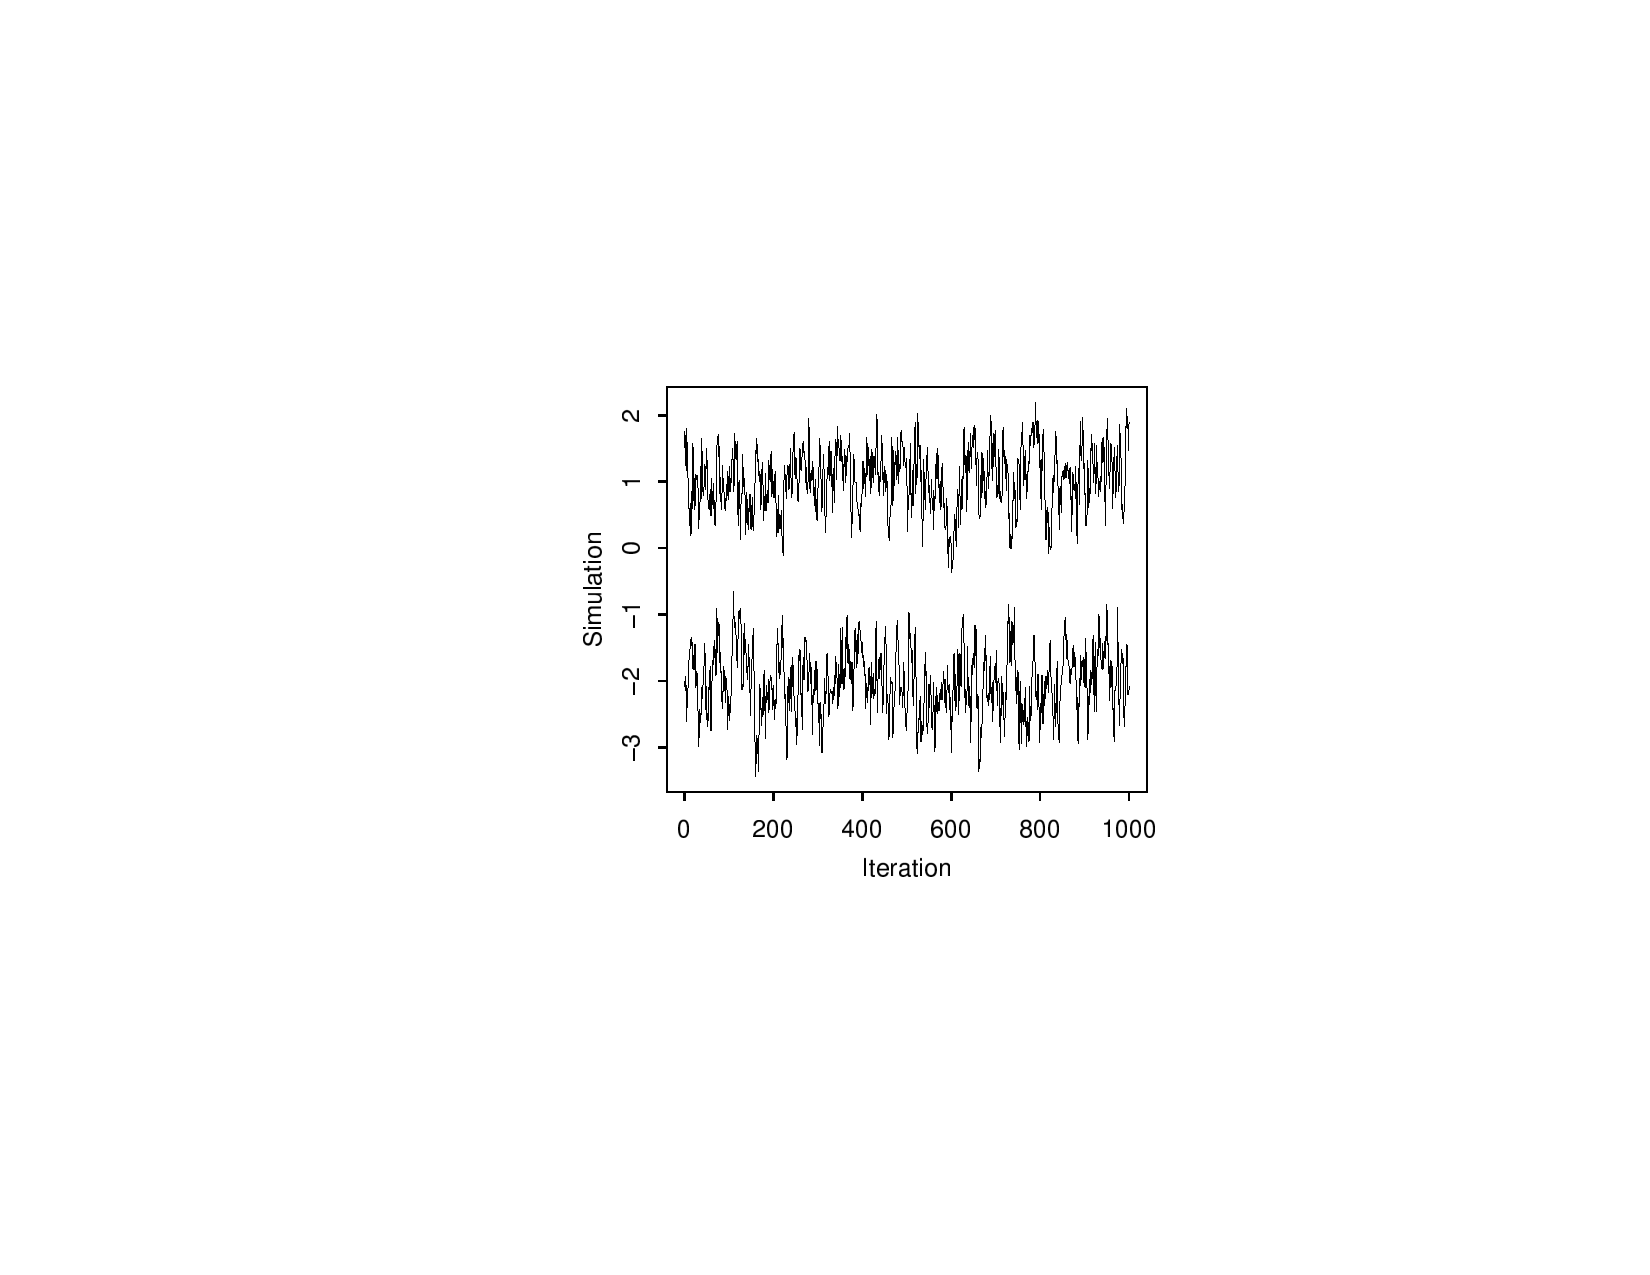
\includegraphics[width=\textwidth]{convergechallenge1.pdf}\hspace{-.5\textwidth}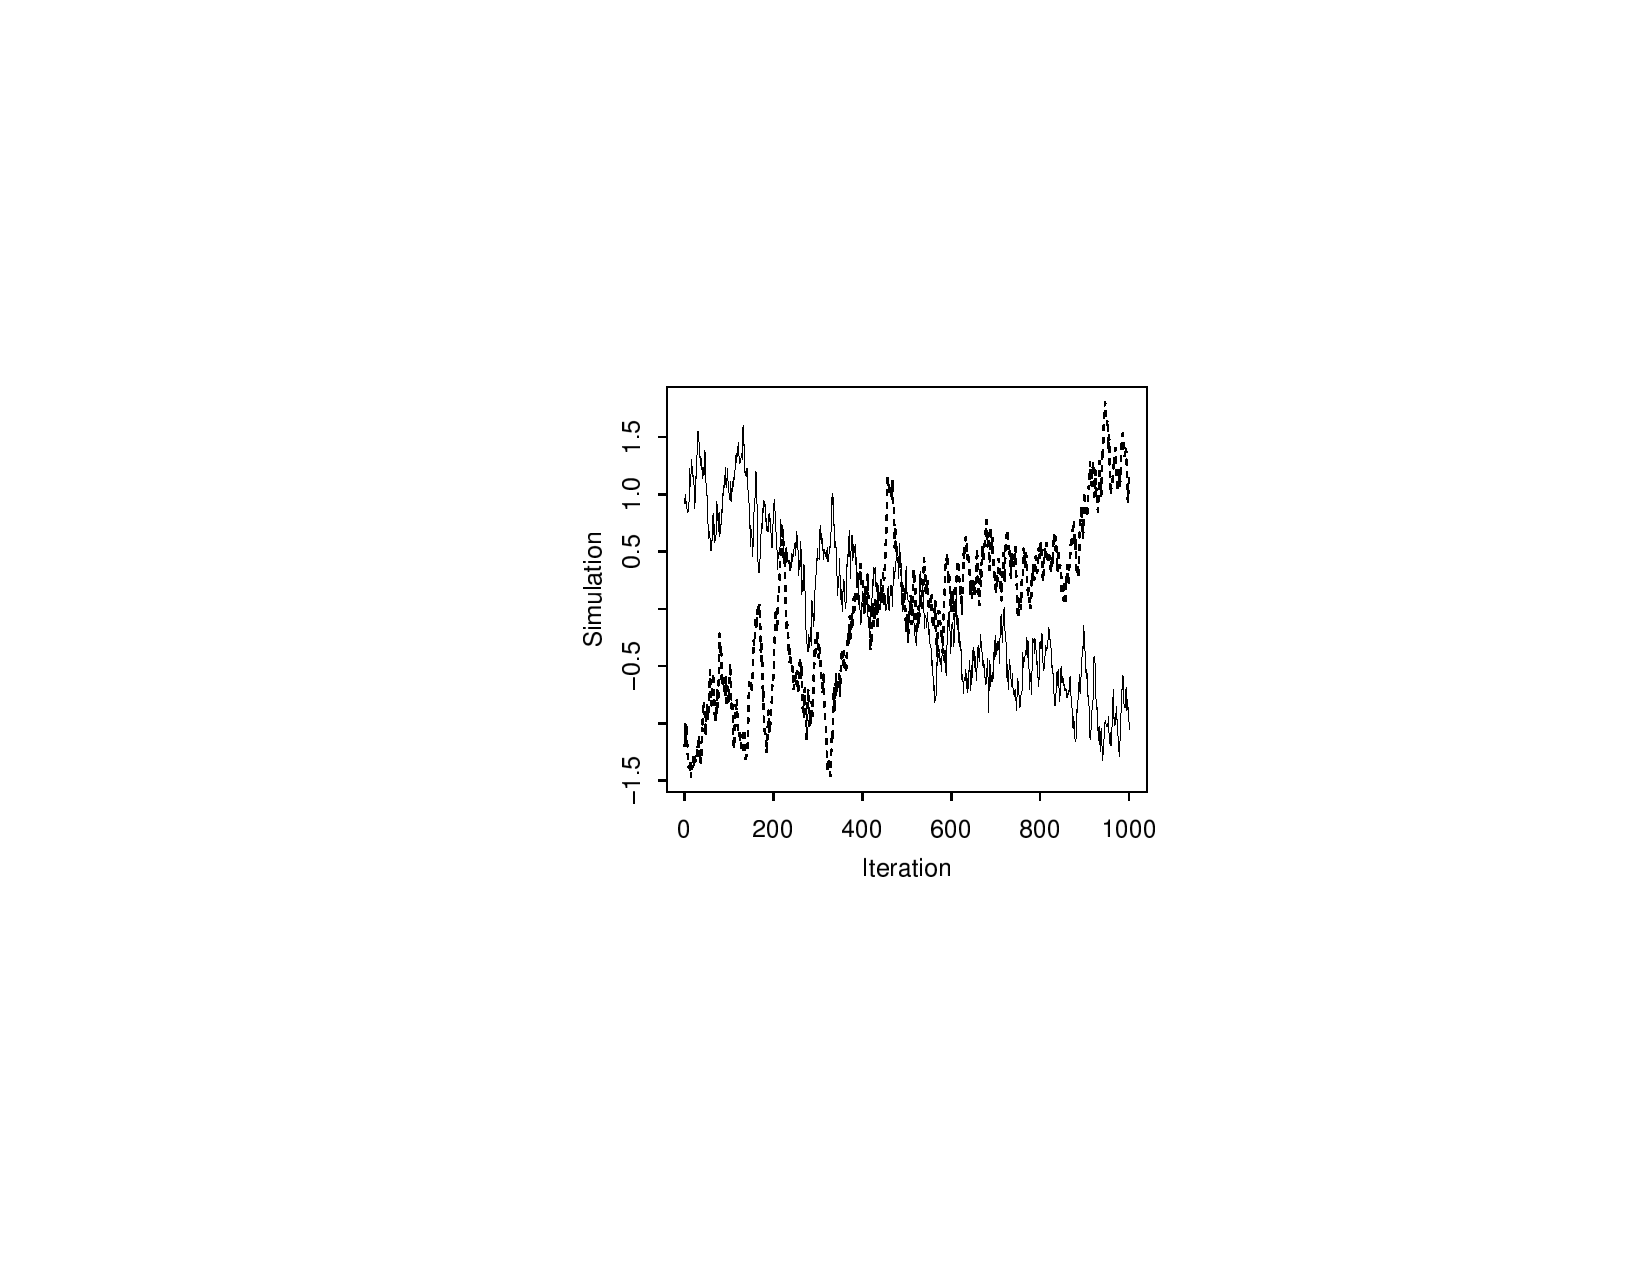
\includegraphics[width=\textwidth]{convergechallenge2.pdf}}
\vspace{-.22\textwidth}
\caption{\em Examples of two challenges in assessing convergence of iterative simulations.  (a) In the left plot, either sequence alone looks stable, but the juxtaposition makes it clear that they have not converged to a common distribution. (b) In the right plot, the two sequences happen to cover a common distribution but neither sequence appears stationary.   These graphs demonstrate the need to use between-sequence and also within-sequence information when assessing convergence. From Gelman et al.\ (2013).}
\label{converge.challenge}
\end{figure}


\section{Splitting each sequence into two parts}
\label{splitting}

We diagnose convergence by splitting each chain in half and checking that all the resulting half-sequences have
mixed.  This simultaneously tests mixing (if all the chains have
mixed well, the separate parts of the different chains should also
mix) and stationarity (at stationarity, the first and second half of
each sequence should be traversing the same distribution).

We start with some number of simulated sequences in which the warm-up period (see Section~\ref{warmup}) has already been discarded.  We then take each of these post-warmup chains and split into the first and second half.  Let $m$ be the number of chains (after splitting) and $n$ be the length of each chain.  We always simulate at least two sequences so that we can observe mixing; see Figure \ref{converge.challenge}a; thus $m$ is always at least 4.  Then for each scalar summary $\psi$, we have a matrix of simulations, $\psi_{ij}$, for $i=1,\dots,n$ and $j=1,\ldots,m$.

\section{Split R-hat}\label{split}

Gelman and Rubin (1992) and Brooks and Gelman (1998) introduced a method for monitoring mixing, using the ratio of between and within-sequence variances of the simulations.  The square root of this ratio is called $\widehat{R}$, or the {\em potential scale reduction factor}.  For example, if $\widehat{R}=2$ for a particular summary $\psi$, this says that the variance of the simulations of $\psi$ in all the chains mixed together is 4 times the average of the within-chain variances of $\psi$.  The implication is that  any given chain is covering only about half the range of all the chains together, and that running the simulations to convergence could reduce the range of $\psi$ by as much as a factor of 2.

In practice, it is common to not consider a set of simulations to have converged until $\widehat{R}$ is less than 1.1 for all parameters in the model, following the reasoning that if $\widehat{R}>1.1$ for any parameter, problems remain with mixing, and inferences might appreciably change if the simulations are run further.

Here are the formulas, with the presentation taken from Gelman et al.\ (2013).  For each scalar summary of interest $\psi$, we compute $B$ and $W$, the between- and within-sequence variances:
\begin{eqnarray*}
B \!\!&=&\!\!
 \frac{n}{m-1}\sum_{j=1}^{m}(\overline{\psi}_{.j}-\overline{\psi}_{..})^2,
\;\mbox{ where }\;\;\overline{\psi}_{.j}=\frac{1}{n}\sum_{i=1}^n \psi_{ij},\;\;
\;\;\overline{\psi}_{..} = \frac{1}{m}\sum_{j=1}^m\overline{\psi}_{.j}\\
W \!\!&=&\!\!
 \frac{1}{m}\sum_{j=1}^{m}s_j^2, \;\mbox{ where }\;\; s_j^2=\frac{1}{n-1}
\sum_{i=1}^n (\psi_{ij}-\overline{\psi}_{.j})^2.
\end{eqnarray*}
The between-sequence variance, $B$, contains a factor of $n$ because it is based on the variance of the within-sequence means, $\overline{\psi}_{.j}$, each of which is an average of $n$ values $\psi_{ij}$.
% If only one sequence is simulated (that is, if $m\!=\!1$), then $B$ cannot be calculated.

We can estimate $\mbox{var}(\psi|y)$, the marginal posterior variance of the estimand, by a weighted average of $W$ and $B$, namely
\begin{equation}\label{hatsig}
\widehat{\mbox{var}}^+(\psi|y)=\frac{n-1}{n}W + \frac{1}{n}B.
\end{equation}
This quantity {\em overestimates}
the marginal posterior variance assuming the starting distribution
is appropriately overdispersed, but is {\em unbiased} under
stationarity (that is, if the starting distribution equals the target
distribution), or
in the limit $n\rightarrow\infty$.
To have overdispersed starting distribution, independent Markov chains
should be initialized with diffuse starting values for the parameters.

Meanwhile, for any finite $n$, the ``within'' variance
$W$ should be an {\em underestimate}
of $\mbox{var}(\psi|y)$ because the individual sequences have not had
time to range over all of the target distribution and, as a result,
will have less variability; in the limit as $n\rightarrow\infty$, the
expectation of $W$ approaches $\mbox{var}(\psi|y)$. The idea to monitor variance across multiple chains comes from Fosdick (1959); the contribution of Gelman and Rubin (1992) was to compare this to within-chain variance.


We monitor convergence of the iterative simulation by estimating
the factor by which the scale of the current distribution for $\psi$
might be reduced if the simulations were continued in the limit
$n\rightarrow\infty$.  This potential scale reduction is estimated for monitoring convergence of iterative simulation by
\begin{equation}\label{rhat.defined}
\widehat{R}=
\sqrt{\frac{\widehat{\mbox{var}}^+(\psi|y)}{W}},
\end{equation}
which declines to 1 as $n\rightarrow\infty$.

We call this {\em split}-$\widehat{R}$ because we are applying it to chains that have already been split in half, as described in Section \ref{splitting}.  Without splitting, $\widehat{R}$ would get fooled by nonstationary chains such as those in Figure \ref{converge.challenge}b.

\paragraph{Rank normalization}

{\em Split}-$\widehat{R}$ assumes that the quantities being considered
have finite mean and variance.  It is also more stable close to
Gaussian the distribution is.  Target distribution can be far from
normal and for example Cauchy distribution has undefined mean and
infinite variance, and thus {\em split}-$\widehat{R}$ is not well
defined. To alleviate thos we propose to compute {\em Split}-$\widehat{R}$
using rank normalized values.

Explain rank-normalization here.

\paragraph{Folded split}

{\em Split}-$\widehat{R}$ can miss if chains have different scales but
have the same location. To alleviate this we propose to to compute
{\em Split}-$\widehat{R}$ also for folded rank normalized values.

Folded values are obtained by transformation
\begin{equation}
  {\mathrm abs}(y-{\mathrm median}(y)).
\end{equation}

\section{Effective sample size}
If the $n$ simulation draws within each sequence were truly
independent, then the between-sequence variance $B$ would be an unbiased
estimate of the posterior variance, $\mbox{var}(\psi|y)$, and we would have
a total of $mn$ independent simulations from the $m$
sequences.  In general, however, the simulations of $\psi$ within each
sequence will be autocorrelated, and $B$ will be larger than $\mbox{var}(\psi|y)$,
in expectation.

A nice introductory reference for analyzing MCMC results in general
and effective sample size in particular is (Geyer, 2011).  The
particular calculations used by Stan follow those for split-$\hat{R}$,
which involve both cross-chain (mean) and within-chain calculations
(autocorrelation); they were introduced in Stan manual and explained
in more detail in Gelman et al. (2013).

One way to define effective sample size for correlated simulation draws is to consider the statistical efficiency of the average of the simulations $\bar{\psi}_{..}$, as an estimate of the posterior mean, $\mbox{E}(\psi|y)$.  This can be a reasonable baseline even though is not the only possible summary and might be inappropriate, for example, if there is particular interest in accurate representation of low-probability events in the tails of the distribution.

The effective sample size of a sequence is defined in terms of the
autocorrelations within the sequence at different lags.  The
autocorrelation $\rho_t$ at lag $t \geq 0$ for a chain with joint
probability function $p(\theta)$ with mean $\mu$ and variance
$\sigma^2$ is defined to be
\begin{equation}
\rho_t
=
\frac{1}{\sigma^2} \, \int_{\Theta} (\theta^{(n)} - \mu)
(\theta^{(n+t)} - \mu) \, p(\theta) \, d\theta.
\end{equation}
This is just the correlation between the two chains offset by $t$
positions.  Because we know $\theta^{(n)}$ and $\theta^{(n+t)}$ have
the same marginal distribution in an MCMC setting, multiplying the
two difference terms and reducing yields
\begin{equation}
\rho_t
=
\frac{1}{\sigma^2} \, \int_{\Theta} \theta^{(n)} \, \theta^{(n+t)} \, p(\theta) \, d\theta.
\end{equation}

The effective sample size of $N$ samples generated by a process with
autocorrelations $\rho_t$ is defined by
\begin{equation}
N_{\mbox{\scriptsize eff}}
\ = \
\frac{N}{\sum_{t = -\infty}^{\infty} \rho_t}
\ = \
\frac{N}{1 + 2 \sum_{t = 1}^{\infty} \rho_t}.
\end{equation}

Effective sample size $N_{\mbox{\scriptsize eff}}$ can be larger than
$N$ in case of antithetic Markov chains, which have negative
autocorrelations on odd lags. Dynamic Hamiltonian algorithm used in Stan can
produce $N_{\mbox{\scriptsize eff}}>N$ for parameters which have close
to Gaussian posterior with low dependency on other parameters.

\subsection{Estimation of Effective Sample Size}

In practice, the probability function in question cannot be tractably
integrated and thus the autocorrelation cannot be calculated, nor the
effective sample size.  Instead, these quantities must be estimated
from the samples themselves.  The rest of this section describes a
autocorrelations and split-$\hat{R}$ based effective sample
size estimator, based on multiple chains. For simplicity, each chain
$\theta_m$ will be assumed to be of length $N$.

Stan carries out the autocorrelation computations for all lags
simultaneously using Eigen's fast Fourier transform (FFT) package with
appropriate padding; see (Geyer, 2011) for more detail on using
FFT for autocorrelation calculations.
%
The autocorrelation estimates $\hat{\rho}_{t,m}$ at lag $t$ from
multiple chains $m \in (1,\ldots,M)$ are combined with within-sample variance estimate $W$ 
and multi-chain variance estimate
$\widehat{\mbox{var}}^{+}$ introduced in the previous section to compute the combined autocorrelation at lag $t$ as
\begin{equation}
\hat{\rho}_t
= 1 - \frac{\displaystyle W - \textstyle \frac{1}{M}\sum_{m=1}^M \hat{\rho}_{t,m}}{\widehat{\mbox{var}}^{+}}. \label{rhohat}
\end{equation}
If the chains have not converged, the variance estimator
$\widehat{\mbox{var}}^{+}$ will overestimate variance, leading to an
overestimate of autocorrelation and an underestimate effective sample
size.

Because of the noise in the correlation estimates $\hat{\rho}_t$ as
$t$ increases, typical truncated sum of $\hat{\rho}_t$ is used.
Negative autocorrelations can happen only on odd lags and by summing
over pairs starting from lag 0, the paired autocorrelation is
guaranteed to be positive, monotone and convex modulo estimator noise
(Geyer, 1992; Geyer, 2011).  Stan uses Geyer's initial monotone
sequence criterion. The effective sample size estimator is defined as
\begin{equation}
\hat{N}_{\mbox{\scriptsize eff}}
=
\frac{MN}
     {\hat{\tau}},
\end{equation}
%
where
\begin{equation}
\hat{\tau} = 1 + 2 \sum_{t=1}^{2m+1} \hat{\rho}_t = -1 + 2 \sum_{t'=0}^{m} \hat{P}_{t'},
\end{equation}
where $\hat{P}_{t'}=\hat{\rho}_{2t'}+\hat{\rho}_{2t'+1}$. Initial
positive sequence estimators is obtained by choosing the largest $m$
such that $\hat{P}_{t'}>0, \quad t' = 1,\ldots,m$. The initial monotone
sequence is obtained by further reducing $\hat{P}_{t'}$ to the minimum
of the preceding ones so that the estimated sequence is monotone.


Our $\hat{n}_{\rm eff}$ is slightly different from similar formulas in the literature in that we use also between-sequence variance in the ratio of (\ref{rhohat}) which typically gives us more conservative claims (lower values of $n_{\rm eff}$) compared to purely between-sequence estimates, especially when mixing is poor. If the chains are not mixing at all (e.g. the posterior is multimodal and the chains are stuck in different modes), then our $\hat{n}_{\rm eff}$ is close to the number of chains.

\paragraph{Rank normalization}

Variance and autocovariance estimates assume also finite mean and variance, and thus as for 
{\em Split}-$\widehat{R}$, we propose to use rank normalization. Effective sample size estimate has been used to adjust the Monte Carlo error estimate of the expectation. We now intentionally separate MCMC diagnostic based on generic and stable rank-normalized relative efficiency $\hat{n}_{\rm eff}/n$ and Monte Carlo error estimates for the desired expectations, which would require also estimation whether mean and variance exist.

We also propose local relative efficiency.

\section{Diagnostics based on Metropolis and HMC dynamics}

$\widehat{R}$ and $n_{\rm eff}$ are entirely based on empirical output and treat the target distribution and the simulation algorithm as black boxes. There are well known cases where {\em split}-$\widehat{R}$ indicates convergence, but all chains have difficulties of reaching some part of the parameter space leading to biased estimates.

Another way to proceed is to monitor convergence to known properties of the target distribution.  Fan, Brooks, and Gelman (2006) suggest an approach based on the score statistic, $U(\theta) = d\log(p(\theta|y))/d\theta$, which has expectation zero under the target distribution.  Thus, it should be possible to diagnose poor convergence if the empirical average of the score statistic computed from the simulation draws is not close to zero.  A related idea is to compare the marginal distribution of a parameter estimated using empirical simulation draws to the estimate from path sampling.  Again, the potential advantage of these methods is they are is using additional information---the gradient of the logarithm of the target density---which is not used by $\widehat{R}$ and $n_{\rm eff}$.  In practice we have not found these diagnostics to be useful, but given that Stan is already computing the gradient in question, maybe it's worth trying them out.
%TODO: not for this paper? remove?

Another direction in diagnostics is to use information such as acceptance rates, jumping distances, and Hamiltonian trajectories that are specific to the simulation algorithm, either with the goal of computing invariants and comparing them to their value under convergence, or monitoring them to detect potential inefficiencies.  It seems natural to examine this sort of diagnostics, given that we are already using the relevant information when tuning the algorithms.  Betancourt (2016, 2017) presents some ideas for Hamiltonian Monte Carlo diagnostics using tree depth, the Bayesian fraction of missing information, and divergences.

\section{Comparisons to other approaches}

It is traditional in systems such as the R package Coda (Plummer et al.~2006) to calculate the effective sample size independently for each chain then sum the result.  In cases where the chains have not converged according to $\widehat{R}$, this induces bias in the form of systematically overestimated effective sample sizes.

It is also common to employ a less conservative stopping method for calculating effective sample sizes.  This will lead to biased estimates that systematically underestimate long-term autocorrelation and thus overestimate effective sample size.

The recommendations provided here are implemented as part of all of the Stan interfaces.

\section{Computational concerns}

Although computation of split-$\widehat{R}$ appears computationally intensive, once the chains have been constructed, it can be carried out with high numerical precision in a single pass over the data using Welford's algorithm with one global accumulator and one for each chain (Welford 1962).  Without splitting, $\widehat{R}$ may be computed entirely online; with split-$\widehat{R}$, at least half the data must be retained in memory.

After split-$\widehat{R}$ has been calculated, the marginal posterior of the estimand, $\widehat{\mathrm{var}}^+(\psi | y)$, will be available.  This leaves only the lagged autocorrelations $\rho_t$, which must be computed for a large number of lags $t$. This can all be carried out with a discrete fast Fourier transform (FFT) by applying the the (discrete) correlation theorem to autocorrelation (Brigham 1974).

\subsection{Generalized $\hat{R}$ for Ragged Chains}

Now suppose that each chain may have a different number of samples.
Let $N_m$ be the number of samples in chain $m$.  Now the formula for
the within-chain mean for chain $m$ uses the size of the chain, $N_m$,
\[
\bar{\theta}_m^{(\bullet)}
= \frac{1}{N_m} \sum_{n = 1}^N \theta^{(m)}_n,
\]
as does the within-chain variance estimate,
\[
s_m^2 = \frac{1}{N_m-1} \, \sum_{n=1}^{N_m} (\theta^{(n)}_m - \bar{\theta}^{(\bullet)}_m)^2.
\]
The terms that average over chains, such as
$\bar{\theta}^{(\bullet)}_{\bullet}$, $B$, and $W$, have the same
definition as before to ensure that each chain has the same effect on
the estimate.  If the averages were weighted by size, a single long
chain would dominate the statistics and defeat the purpose of
monitoring convergence with multiple chains.

Because it contains the term $N$, the estimate $\widehat{var}^{+}$
must be generalized.  By expanding the first term,
\[
\frac{N-1}{N}\, W \,
\ = \
\frac{N-1}{N} \frac{1}{M} \, \sum_{m=1}^M
\frac{1}{N-1} \, \sum_{n=1}^N (\theta^{(n)}_m -
\bar{\theta}^{(\bullet)}_m)^2
\ = \
\frac{1}{M}
\sum_{m=1}^M
\frac{1}{N}
\sum_{n=1}^N (\theta^{(n)}_m -
\bar{\theta}^{(\bullet)}_m)^2,
\]
and the second term,
\[
\frac{1}{N}\, B
\ = \
\frac{1}{M-1} \, \sum_{m=1}^M (\bar{\theta}^{(\bullet)}_{m} - \bar{\theta}^{(\bullet)}_{\bullet})^2.
\]
the variance estimator naturally generalizes to
\[
\widehat{\mbox{var}}^{+}\!(\theta|y)
=
\frac{1}{M}
\sum_{m=1}^M
\frac{1}{N_m}
\sum_{n=1}^{N_m} (\theta^{(n)}_m -
\bar{\theta}^{(\bullet)}_m)^2
+
\frac{1}{M-1} \, \sum_{m=1}^M (\bar{\theta}^{(\bullet)}_{m} -
\bar{\theta}^{(\bullet)}_{\bullet})^2.
\]
%
If the chains are all the same length, this definition is equivalent
to the one in the last section.  This generalized variance estimator
and the within-chains variance estimates may be plugged directly into
the formula for $\hat{R}$ from the previous section.

\section{Related issues and open questions}

\label{warmup}Algorithms such as Metropolis and Hamiltonian Monte Carlo require tuning, and these tuning operations typically destroy the conditions under which the stationary distribution of the algorithm equals the target distribution.  Se we discard the simulations obtained during this {\em warmup} period.  A practical question then arises:  how long should the warm-up period be, and how long should we run the simulations after warmup?  By default Stan currently runs 4 parallel chains from different starting points, with 1000 warmup iterations in which there is adaptation of the Hamiltonian Monte Carlo mass matrix, followed by 1000 more iterations on each chain.  The result is then 4 chains of 1000 saved iterations each, which after splitting yield 8 chains each of length 500 for the computation of $\widehat{R}$.

Some questions for further research include the possibility of the length of the warmup itself being adaptive, and also the possibility of choosing how long to run the computation based on wall time rather than a fixed number of iterations.  One minor complication is that this leads to ``ragged'' arrays of simulations, with different chains of different lengths, so that the formulas for $\widehat{R}$ and $n_{\rm eff}$ must be altered slightly.  Options then arise as to how to weight the various chains, with extremes being chains weighted equally and draws weighted equally; see Stan Development Team (2017).




For models with many parameters, the computations of $\widehat{R}$ and $n_{\rm eff}$ are not free.  There may be more efficient ways to compute these than just using the simple formulas above.  Another challenge is computing these as the algorithm is running.  Suppose, for example, one wanted to run the simulations until $\widehat{R}<1.05$ for all parameters.  It could be expensive to recompute this every step.  While $\widehat{R}$ is easy to compute as draws come in using Welford's algorithm.  The splitting introduces a complication in that, with every two new iterations in a chain, we need to transfer one iteration from the second half to the first half;  it is still possible to compute online, but it requires at least half the chain to be buffered.

Split $\widehat{R}$ is kind of a hack.  We can perhaps envision some more general idea, perhaps something FFT-like, that splits the chains into subsequences of length $n/2, n/4, n/8$, and so forth.

Brooks and Gelman (1998) introduce a multivariate potential scale reduction factor, a generalization of $\widehat{R}$ that compares between- and within-chain covariance matrices of the simulation draws.  We never really explored this idea because when we tried it, multivariate $\widehat{R}$ was staying large even after it seemed that the chains were mixing well.  So there seemed to be problems with $\widehat{R}$ as a practical tool as it was so conservative.  But maybe this is worth looking into further.  While this can also be computed online, the downside is that it requires a quadratic amount of arithmetic per draw to update all the covariances.

Brooks and Gelman (1998) also introduce nonparametric versions of $\widehat{R}$; there are lots of ideas here, for example for each scalar summary $\phi$ computing the central 80\% interval from each chain alone, and then summarizing by the average coverage of these separate intervals with respect to the distribution of all the chains mixed together.  This measure has the advantage of being on the scale of coverage; also it uses quantiles rather than averages and variances, so it will work for long-tailed distributions such as the Cauchy where $\widehat{R}$ would fail.

Yet another direction is to use graphical diagnostics, including traceplots of multiple chains and visualizations of Hamiltonian trajectories.  For reasons noted at the end of Section \ref{intro}, we need automatic numerical measures that will flag potential problems; at that point graphical methods such as in ShinyStan (Gabry, 2017) can be helpful in understanding how to move forward.

\section*{References}

\noindent

\bibitem Betancourt, M. (2016).  Diagnosing suboptimal cotangent disintegrations in Hamiltonian Monte Carlo. \url{https://arxiv.org/abs/1604.00695}

\bibitem Betancourt, M. (2017).  Robust statistical workflow with RStan.  \url{http://mc-stan.org/users/documentation/case-studies/rstan_workflow.html}

\bibitem Brigham, E. O. (1974). {\em The Fast Fourier Transform}.  Englewood Cliffs, New Jersey: Prentice Hall.

\bibitem Brooks, S. P., and Gelman, A. (1998).  General methods for monitoring convergence of iterative simulations.  {\em Journal of Computational and Graphical Statistics} {\bf 7}, 434--455.

\bibitem Brooks, S., Gelman, A., Jones, G. L., and Meng, X. L., eds.\ (2011).  {\em Handbook of Markov Chain Monte Carlo}.  London:  CRC Press.

\bibitem Fan, Y., Brooks, S., and Gelman, A. (2006).  Output assessment for Monte Carlo simulations via the score statistic. {\em Journal of Computational and Graphical Statistics} {\bf 15}, 178--206.

\bibitem Fosdick, L. D. (1959).  Calculation of order parameters in a binary alloy by the Monte Carlo method. {\em Physical Review} {\bf 116}, 565--573.

\bibitem Gabry, S. (2017).  ShinyStan:  Analysis \& visualization GUI for MCMC.  \url{http://mc-stan.org/users/interfaces/shinystan.html}

\bibitem Gabry, J., Simpson, D., Vehtari, A., Betancourt, M., and Gelman, A. (2018). Visualization in Bayesian workflow. {\em Journal of the Royal Statistical Society Series A}, accepted for publication.
  
\bibitem Gelman, A., Carlin, J. B., Stern, H. S., Dunson, D. B., Vehtari, A. and Rubin, D. B. (2013). {\em Bayesian Data Analysis}, third edition. London:  CRC Press.

\bibitem Gelman, A., and Rubin, D. B. (1992a).  A single sequence from the Gibbs sampler gives a false sense of security.
In {\em Bayesian Statistics 4}, ed.\ J. M. Bernardo, J. O. Berger, A. P. Dawid, and A. F. M. Smith, 625--631.  Oxford University Press.

\bibitem Gelman, A., and Rubin, D. B. (1992b).   Inference from iterative simulation using multiple sequences (with discussion).  {\em Statistical Science} {\bf 7}, 457--511.

\bibitem Geyer, C. J. (1992). Practical {Markov} Chain {Monte} {Carlo} (with discussion). {\em Statistical Science}, {\bf 7}, 473--483.

\bibitem Geyer, C. J. (2011). Introduction to Markov chain Monte Carlo. In {\em Handbook of Markov Chain Monte Carlo}, ed.\ Brooks, S., Gelman, A., Jones, G. L., and Meng, X. L., 3--48.  London:  CRC Press.

\bibitem Plummer, M., Best, N., Cowles, K. and Vines, K., (2006). CODA: convergence diagnosis and output analysis for MCMC. {\em R news} 6(1):7--11.

\bibitem Stan Development Team (2017). Stan: A C++ library for probability and sampling, version 2.16.0.   \url{http://mc-stan.org}

\bibitem Welford, B. P. (1962). Note on a method for calculating corrected sums of squares and products. {\em Technometrics} 4(3):419--420.

\end{document}


